% Copyright 2004 by Till Tantau <tantau@users.sourceforge.net>.
%
% In principle, this file can be redistributed and/or modified under
% the terms of the GNU Public License, version 2.
%
% However, this file is supposed to be a template to be modified
% for your own needs. For this reason, if you use this file as a
% template and not specifically distribute it as part of a another
% package/program, I grant the extra permission to freely copy and
% modify this file as you see fit and even to delete this copyright
% notice. 

\documentclass[aspectratio=169]{beamer}
%\documentclass{beamer}

\setbeamersize{text margin left=5mm, text margin right=5mm}


\defbeamertemplate{headline}{my header}{%
\vskip1pt%
\makebox[0pt][l]{\,\insertshortauthor}%
\hspace*{\fill}\insertshorttitle/\insertshortsubtitle\hspace*{\fill}%
\llap{\insertpagenumber/\insertpresentationendpage\,}
}
\setbeamertemplate{headline}[my header]

\let\olditem\item
\renewcommand{\item}{\setlength{\itemsep}{\fill}\olditem}

\usepackage{soul}
\usepackage{tkz-euclide}
\usetikzlibrary{calc}
\usepackage[]{algorithm2e}
\usepackage{changepage}
\usepackage{amssymb}
\usepackage{xcolor}
\usepackage{mathtools}
\usepackage{tcolorbox}
\usepackage{tikz}
\usepackage{tikz-3dplot}
\usepackage[export]{adjustbox}
\usepackage{tabu}

% \usepackage[math]{cellspace}
% \cellspacetoplimit 4pt
% \cellspacebottomlimit 4pt
%\usetikzlibrary{arrows.meta}

%\setbeamertemplate{itemize items}{-}

%\usepackage{helvet}
\usefonttheme{professionalfonts} % using non standard fonts for beamer
%\usefonttheme{serif} % default family is serif
%\usepackage{fontspec}
%\setmainfont{Liberation Serif}

% There are many different themes available for Beamer. A comprehensive
% list with examples is given here:
% http://deic.uab.es/~iblanes/beamer_gallery/index_by_theme.html
% You can uncomment the themes below if you would like to use a different
% one:
%\usetheme{AnnArbor}
%\usetheme{Antibes}
%\usetheme{Bergen}
%\usetheme{Berkeley}
%\usetheme{Berlin}
%\usetheme{Boadilla}
%\usetheme{boxes}
%\usetheme{CambridgeUS}
%\usetheme{Copenhagen}
%\usetheme{Darmstadt}
%\usetheme{default}
%\usetheme{Frankfurt}
%\usetheme{Goettingen}
%\usetheme{Hannover}
%\usetheme{Ilmenau}
%\usetheme{JuanLesPins}
%\usetheme{Luebeck}
%\usetheme{Madrid}
%\usetheme{Malmoe}
%\usetheme{Marburg}
%\usetheme{Montpellier}
%\usetheme{PaloAlto}
%\usetheme{Pittsburgh}
%\usetheme{Rochester}
%\usetheme{Singapore}
%\usetheme{Szeged}
%\usetheme{Warsaw}


\def\mf{\ensuremath\mathbf}
\def\mb{\ensuremath\mathbb}
\def\mc{\ensuremath\mathcal}
\def\lp{\ensuremath\left(}
\def\rp{\ensuremath\right)}
\def\lv{\ensuremath\left\lvert}
\def\rv{\ensuremath\right\rvert}
\def\lV{\ensuremath\left\lVert}
\def\rV{\ensuremath\right\rVert}
\def\lc{\ensuremath\left\{}
\def\rc{\ensuremath\right\}}
\def\ls{\ensuremath\left[}
\def\rs{\ensuremath\right]}
\def\bmx{\ensuremath\begin{bmatrix*}[r]}
\def\emx{\ensuremath\end{bmatrix*}}
\def\bmxc{\ensuremath\begin{bmatrix*}[c]}
\def\t{\lp t\rp}
\def\k{\ls k\rs}


\newcommand{\demoex}[2]{\onslide<#1->\begin{color}{black!60} #2 \end{color}}
\newcommand{\demoexc}[3]{\onslide<#1->\begin{color}{#2} #3 \end{color}}
\newcommand{\anim}[3]{\onslide<#1->{\begin{color}{#2!60} #3 \end{color}}}
\newcommand{\ct}[1]{\lp #1\rp}
\newcommand{\dt}[1]{\ls #1\rs}
\newcommand{\cols}[2]{\begin{columns}[#1] #2 \end{columns}}
\newcommand{\col}[2]{\begin{column}{#1} #2 \end{column}}

\newcommand{\xdownarrow}[1]{%
  {\left\downarrow\vbox to #1{}\right.\kern-\nulldelimiterspace}
}

\title{Introduction to Digital Signal Processing}

% A subtitle is optional and this may be deleted
\subtitle{Z-transform}

\author{Sivakumar Balasubramanian}
% - Give the names in the same order as the appear in the paper.
% - Use the \inst{?} command only if the authors have different
%   affiliation.

\institute[Christian Medical College] % (optional, but mostly needed)
{
  \inst{}%
  Department of Bioengineering\\
  Christian Medical College, Bagayam\\
  Vellore 632002
}
% - Use the \inst command only if there are several affiliations.
% - Keep it simple, no one is interested in your street address.

\date{}
% - Either use conference name or its abbreviation.
% - Not really informative to the audience, more for people (including
%   yourself) who are reading the slides online

\subject{Lecture slides on Introduction to DSP}
% This is only inserted into the PDF information catalog. Can be left
% out. 

% If you have a file called "university-logo-filename.xxx", where xxx
% is a graphic format that can be processed by latex or pdflatex,
% resp., then you can add a logo as follows:

% \pgfdeclareimage[height=0.5cm]{university-logo}{university-logo-filename}
% \logo{\pgfuseimage{university-logo}}

% Delete this, if you do not want the table of contents to pop up at
% the beginning of each subsection:
\AtBeginSubsection[]
{
  \begin{frame}<beamer>{Outline}
    \tableofcontents[currentsection,currentsubsection]
  \end{frame}
}

% Let's get started
\begin{document}

\begin{frame}
  \titlepage
\end{frame}


\begin{frame}[t]{Z transform}
\begin{itemize}
  \item Exponential signals are \textit{eigenfucntiopns} of LTI systems.
  \[  z^n \longrightarrow H\lp z \rp z^n \]
  $H(z)$ is the eigenvalue corresponding to the eigenfunction $z^n$.

  \item If $x[n] = \sum_{k} \alpha_k z_k^n$, then $y[n] = \sum_{k} \alpha_k H\lp z_k \rp z_k^n$.
  \[ \begin{split}
      \lp \alpha_k \rp_{k \in \mb{Z}} & \longrightarrow \text{Representation of } x[n] \text{ using } z_k^n \\
      \lp H\lp z_k \rp \alpha_k \rp_{k \in \mb{Z}} & \longrightarrow \text{Representation of } x[n] \text{ using } z_k^n \\
      \end{split} \]

  \item The z-transoform allows us to find the representation of any disctet-time signal $x[n]$ in terms of the set of complex exponentials $\{ z^n \}_{z \in \mb{C}}$ 
\end{itemize}
\end{frame}


\begin{frame}[t]{z transform}
The z-transform of a discrete time signal $x[n]$ is defined as the following power seris,
\[ X\lp z \rp \triangleq \sum_{n=-\infty}^{\infty} x[n] z^{-n} = \mc{Z}\lp x[n] \rp\]
\[ x[n] \xleftrightarrow{\mc{Z}} X\lp z \rp  \]
where, $z \in \mb{C}$.

\begin{itemize}
  \item The values of $z$ for which the above summation covnerges is called the \textit{region of conergence} of $X(z)$.
\end{itemize}
\end{frame}


\begin{frame}[t]{z transform}
z-transform of some signals.
\begin{enumerate}
  \item $\delta[n]$
  \item $\delta[n-k]$
  \item $\delta[n+k]$
  \item $\sum_{k=0}^{5} \alpha_k \delta[n - k]$
  \item $1[n]$
  \item $a^k \cdot 1[n]$
  \item $-a^{k} \cdot 1[-n-1]$
\end{enumerate}
\end{frame}


\begin{frame}[t]
  \frametitle{z-transform and ROCs}
  \begin{center}
  \begin{figure}
  \centering
  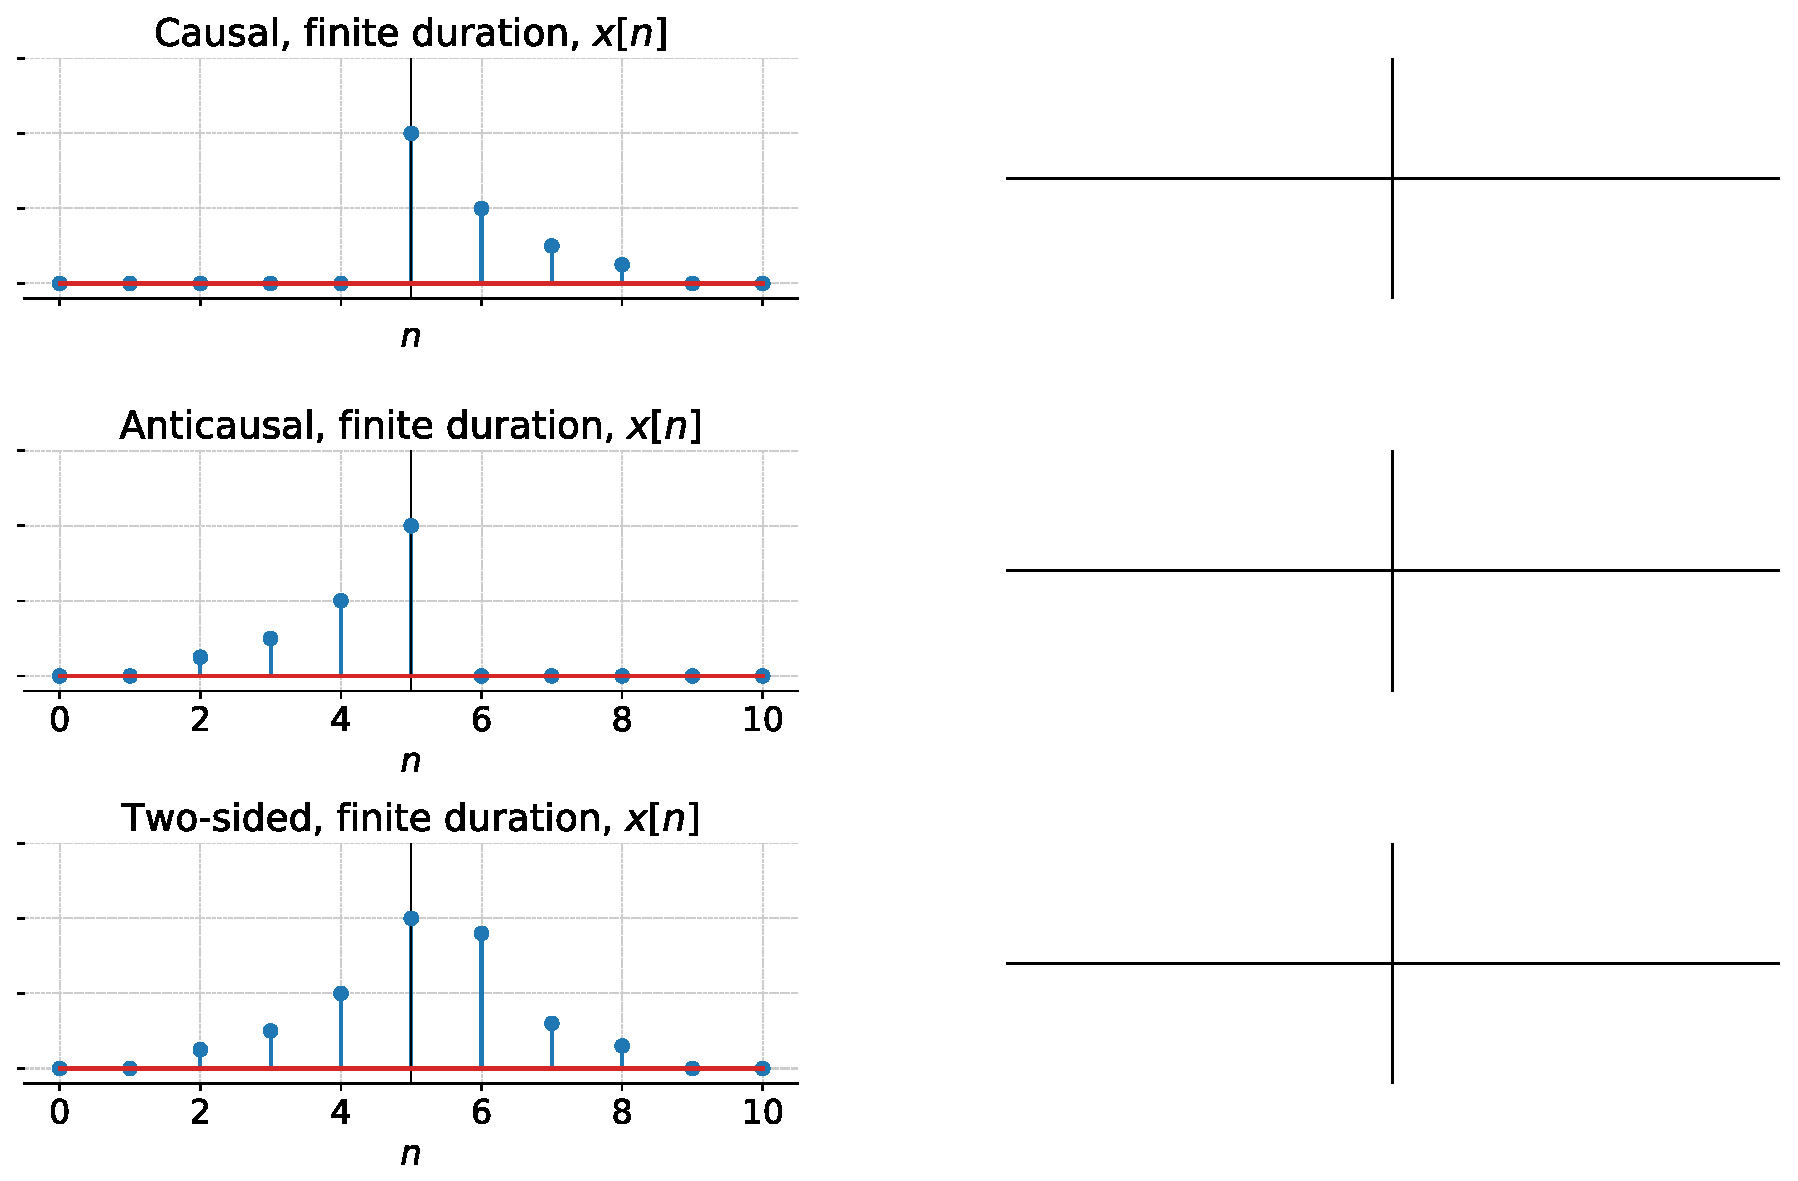
\includegraphics[width=0.7\textwidth, left]{img/ztrans-finite-dur.eps}
  \end{figure}
  \end{center}
\end{frame}


\begin{frame}[t]
  \frametitle{z-transform and ROCs}
  \begin{center}
  \begin{figure}
  \centering
  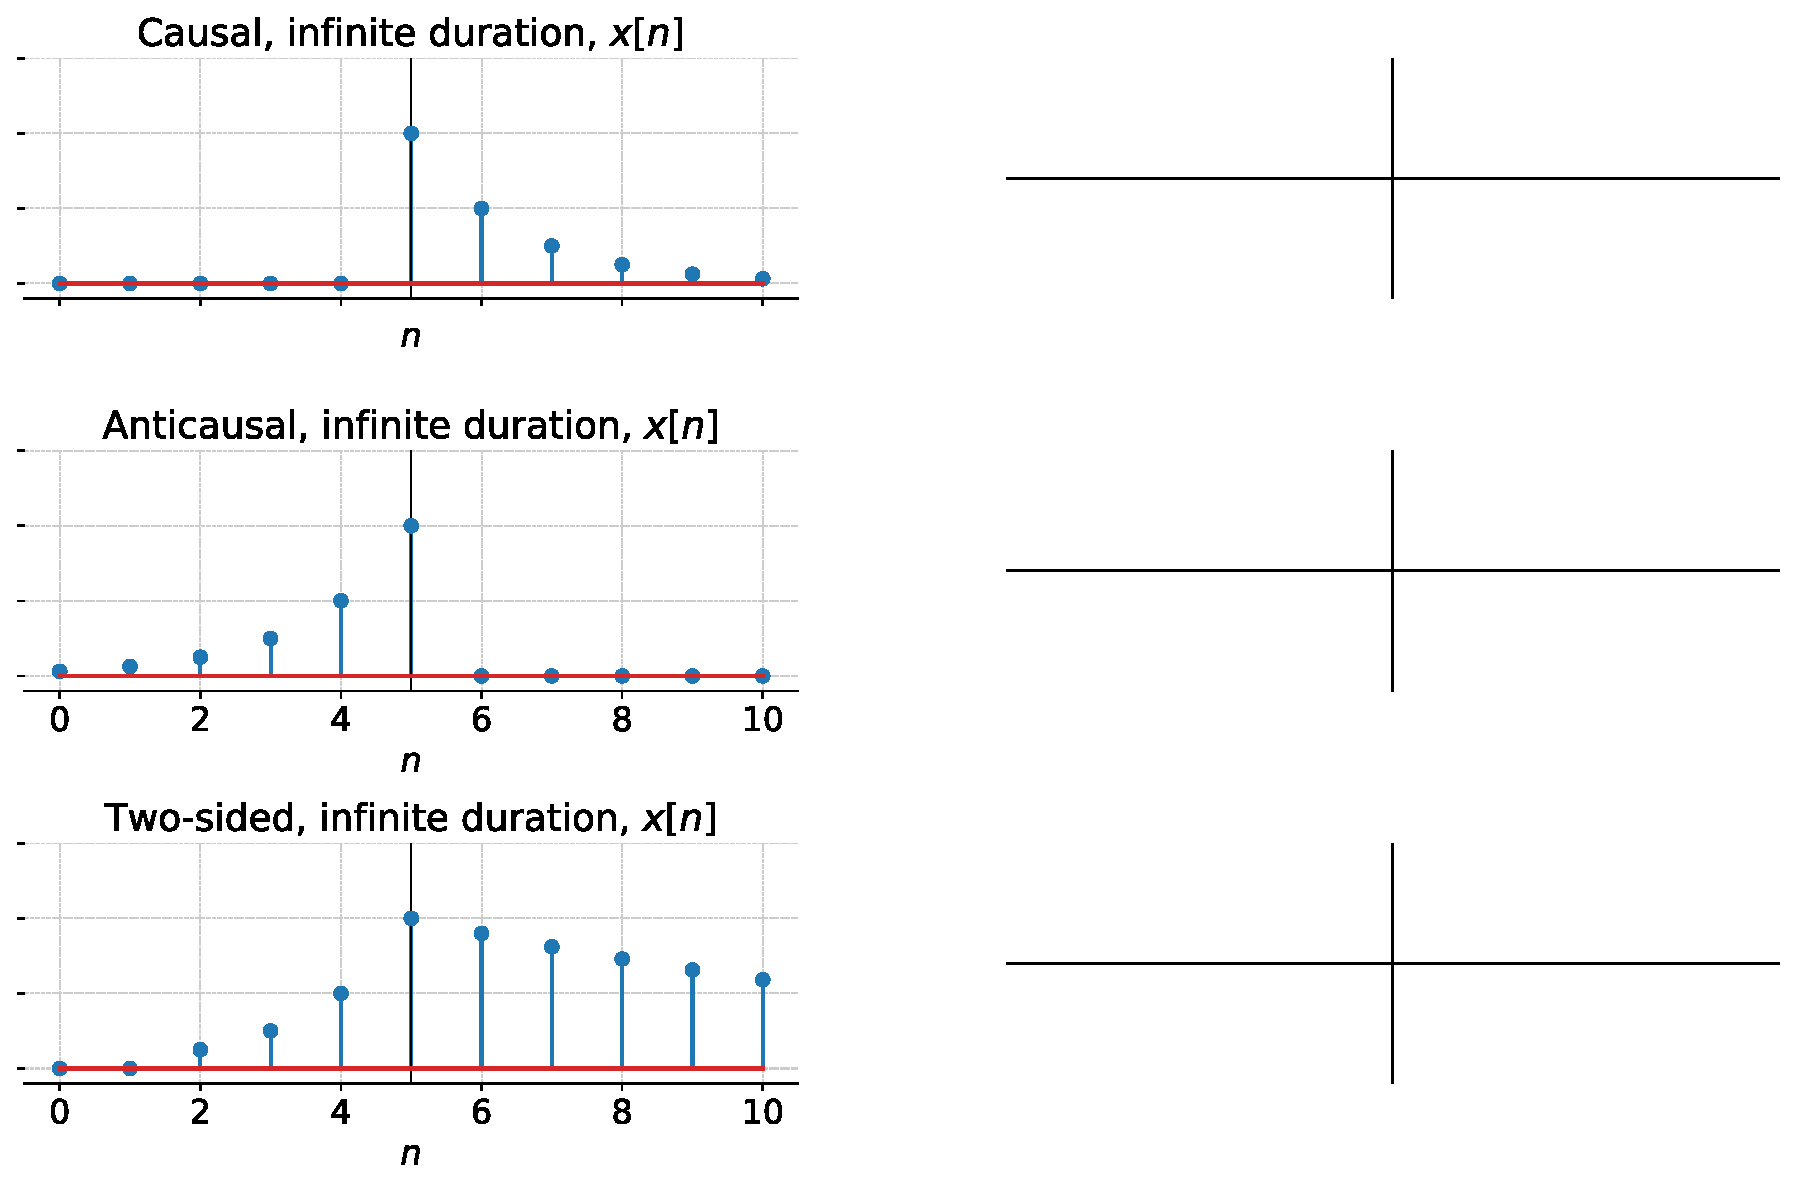
\includegraphics[width=0.7\textwidth, left]{img/ztrans-infinite-dur.eps}
  \end{figure}
  \end{center}
\end{frame}


\begin{frame}[t]
  \frametitle{Properties of the z-transform}
  \begin{itemize}
      \item Linearity
      \item Time-shifting
      \item Convolution in time
      \item Initital value theorem
    \end{itemize}  
\end{frame}

\begin{frame}[t]
  \frametitle{Transfer function of an LTI system}

  The z-transform of the impulse response $h[n]$ is defined as the transfer function of a discrete-time LTI system.
  \[ H\lp z \rp = \sum_{n=-\infty}^{\infty} h[n] z^{-n} \]

  When the system is causal, then $H\lp z \rp = \sum_{n=0}^{\infty} h[n] z^{-n}$.

  The z-transforms of the input $x[n]$ and $y[n]$ are related to each other through the transfer function, 
  \[ Y(z) = H(z) \cdot X(z) \]
\end{frame}

\begin{frame}[t]
  \frametitle{Unilateral z-transform}

  When solving difference equations, we are interested in computing the output $y[n]$ from time $n=0$ for an input $x[n]$ that is specified from time $n=0$. Here we cannot use the regular z-transform (also called as two-sided or bilateral z-transform). 

  \[ X^+(z) \triangleq \sum_{n=0}^{\infty} x[n] z^{-n} \]
  
  This is useful when analysing linear difference equations.

  When the time domain signal $x[n]$ is delayed by a sample, such that the signal is $x[n-1] \cdot 1[n]$, then we have
  \[ x[n] \xleftrightarrow{\mc{Z}^+} X^+(z) \implies x[n-1] \xleftrightarrow{\mc{Z}^+} z^{-1} X^+\lp z \rp + x[-1] \]

  $X^+(z) = X(z)$ for causal an signal $x[n]$.
\end{frame}

\begin{frame}[t]
  \frametitle{Rational z-transforms}
  \begin{itemize}
    \item In practice, we often come across rational polynomial of $z$.
    \item Consider a LTI system described by the following different equation,
    \[ y[n] + a_1 y[n-1] + a_2 y[n-2] + \cdot + a_Ny[n - N] = b_0x[n] + b_1 x[n-1] + \cdots + b_M x[n - M] \] 
    We are interested in sovling this equation from time $n = 0$ for an input specified from time $n \geq 0$. Taking the unilateral z-transform on both sides,
    \[ \begin{split}
        y[n] \xleftrightarrow{\mc{Z}^+} \,\, & \,\, Y^+(z) \\
        y[n-1] \xleftrightarrow{\mc{Z}^+} \,\, & \,\, z^{-1}Y^+(z) + y[-1] \\
        y[n-2] \xleftrightarrow{\mc{Z}^+} \,\, & \,\, z^{-2}Y^+(z) + z^{-1}y[-1] + y[-2] \\
        \vdots & \\
        y[n-N] \xleftrightarrow{\mc{Z}^+} \,\, & \,\, z^{-N}Y^+(z) + z^{-(N-1)}y[-1] + z^{-(N-2)}y[-2] + \cdots + y[-N]
        \end{split} 
        \]
  \end{itemize}
\end{frame}


\begin{frame}[t]
  \frametitle{Rational z-transforms}
  If we assume a causal inout signal $x[n]$,
  \[ Y^+(z) + \sum_{k=1}^N a_kz^{-k} \lp Y^+(z) + \sum_{l=1}^{k} y[-l] z^{l}\rp = X(z)\lp b_0 + b_1z^{-1} + \cdots + z^{-M} \rp\]
  \[ Y^+(z)\lp 1 + \sum_{k=1}^N a_kz^{-k} \rp + \sum_{k=1}^N a_kz^{-k} \lp \sum_{l=1}^{k} y[-l] z^{l} \rp = X(z)\lp b_0 + b_1z^{-1} + \cdots + z^{-M}\rp \]
  \[ Y^+(z) =  \frac{B(z)}{A(z)} X\lp z \rp + \frac{N_0(z)}{A(z)}  \]
  where, 
  \begin{itemize}
    \item $B(z) = \sum_{l=0}^{M} b_l z^-l$
    \item $A(z) = 1 + \sum_{k=1}^N a_kz^{-k}$
    \item $N_0(z) = -\sum_{k=1}^N a_kz^{-k} \lp \sum_{l=1}^{k} y[-l] z^{l} \rp$
  \end{itemize}
\end{frame}


\begin{frame}[t]
  \frametitle{Rational z-transform}
  Zero-state response, when the initial conditions are zero.
  \[ Y_{zs}(z) = \frac{B\lp z \rp}{A\lp z \rp}X\lp z \rp = H\lp z \rp X\lp z \rp \]

  Zero-input reesponse, wheren the input is zero and the initial conditions are non-zero.
  \[ Y_{zi}^+\lp z \rp = \frac{N_0\lp z \rp}{A\lp z \rp} \]
\end{frame}


\begin{frame}[t]
  \frametitle{Inverse z-transform of Rational Polynomials of $z$}
  Consider the following rational polynomial,
  \[ X(z) = \frac{N(z)}{D(z)} = \frac{b_0 + b_1z^{-1} + \cdots + b_Mz^{-M}}{1 + a_1z^{-1} + \cdots + a_Nz^{-N}} \]

  The rational polynomial $X(z)$ is called \textit{proper} if $M < N$ and $a_N \neq 0$.

  It is \textit{improper} if $M \geq N$.

  Improper rationla polynomial can be converted to the following form,
  \[ X(z) = \frac{N(z)}{D(z)} = c_0 + c_1z^{-1} + \cdots + c_{M-N}z^{-(M-N)} + \frac{N_0(z)}{D(z)} \]

  Convert the rational polynomial as a function of $z$ instead of $z^{-1}$ by multiplying both the numerator and denominator by $z^{N}$.
  \[ X(z) = \frac{N(z)}{D(z)} = \frac{b_0z^N + b_1 z^{N-1} + \cdots + b_Mz^{N-M}}{z^N + a_1z^{N-1} + \cdots + a_N} \]
\end{frame}


\begin{frame}[t]
  \frametitle{Inverse z-transform of Rational Polynomials of $z$}
  Convert the rational polynomial as a function of $z$ instead of $z^{-1}$ by multiplying both the numerator and denominator by $z^{N}$.
  \[ X(z) = \frac{N(z)}{D(z)} = \frac{b_0z^N + b_1 z^{N-1} + \cdots + b_Mz^{N-M}}{z^N + a_1z^{N-1} + \cdots + a_N} \]
  \[ \frac{X(z)}{z} = \frac{b_0z^{N-1} + b_1 z^{N-2} + \cdots + b_Mz^{N-M-1}}{z^N + a_1z^{N-1} + \cdots + a_N} \]

  Let the roots of the denominator of $\frac{X(z)}{z}$ be $p_1, p_2, \ldots p_N$.
  \[ \frac{X(z)}{z} = \frac{b_0z^{N-1} + b_1 z^{N-2} + \cdots + b_Mz^{N-M-1}}{\lp z - p_1\rp \lp z - p_2\rp \cdots \lp z - p_N\rp} \]

  The roots of the denominator $D(z)$ are the called the \textit{poles} of $X(z)$ and the roots of the numerator $N(z)$ are called the \textit{zeros} of $X(z)$.
\end{frame}


\begin{frame}[t]
  \frametitle{Inverse z-transform of Rational Polynomials of $z$}
  \textbf{Distinct Poles}
  \[ \frac{X(z)}{z} = \frac{b_0z^{N-1} + b_1 z^{N-2} + \cdots + b_Mz^{N-M-1}}{\lp z - p_1\rp \lp z - p_2\rp \cdots \lp z - p_N\rp} = \frac{A_1}{z - p_1} + \frac{A_2}{z - p_2} + \cdots + \frac{A_N}{z - p_N} \]

  Multipying both sides by $(z - p_k)$, and substituting $z = p_k$, we get
  \[ (z - p_k)\frac{X(z)}{z} \bigg\vert_{z = p_k} = A_k \]

  Find the inverse z-transform of the following,
  \[ X(z)  =\frac{1 + z^{-1}}{1 - z^{-1} + 0.5z^{-2}}\]
\end{frame}


\begin{frame}[t]
  \frametitle{Inverse z-transform of Rational Polynomials of $z$}  
\end{frame}


\begin{frame}[t]
  \frametitle{Inverse z-transform of Rational Polynomials of $z$}
  \textbf{Multiple-order poles}. Let $X(z)$ have a pole of multiplicity $l$, then the denominator has a term $(z - p_k)^l$

  Find the inverse z-transform of the following,
  \[ X(z)  =\frac{1}{(1 + z^{-1})(1 - z^{-1})^2} \]
\end{frame}


\begin{frame}[t]
  \frametitle{Inverse z-transform of Rational Polynomials of $z$}
  \[ \mc{Z}^{-1} \lp \frac{1}{1 - z^{-1}p_k} \rp = \begin{cases}
  p_k^n \cdot 1[n], & ROC: \vert z \vert > \vert p_k \vert \\ 
  -p_k^n \cdot 1[-n-1], & ROC: \vert z \vert < \vert p_k \vert \\ 
  \end{cases} \]  

  When we have multiple poles,
  \[ \mc{Z}^{-1} \lp \frac{pz^{-1}}{(1 - z^{-1}p)^2} \rp = np^n\cdot 1[n] \]  
\end{frame}


\begin{frame}[t]
  \frametitle{Response of LTI systems}
  Let the transfer function of an LTI system be,
  \[ H(z) = \frac{B(z)}{A(z)} \]

  Let the z-transform of the input signal be $X(z) = \frac{N(z)}{Q(z)}$. 

  The output of the system is given by,
  \[ Y(z) = \frac{B(z)N(z)}{A(z)Q(z)} \]

  Assuming there are no repeated poles in the denominator $A(z) Q(z)$,
  \[ Y(z) = \sum_{k=1}^N \frac{A_k}{1 - p_kz^{-1}} + \sum_{k=1}^L \frac{Q_k}{1 - q_kz^{-1}} \]
  \[ y[n] = \sum_{k=1}^N A_k \cdot p_k^n \cdot 1[n] + \sum_{k=1}^N Q_k \cdot q_k^n \cdot 1[n] \]
\end{frame}


\begin{frame}[t]
  \frametitle{Response of LTI systems}
  Find the output of the causal LTI system for zero initial conditions,
  \[ H(z) = \frac{1}{1 - 0.5z^{-1}} \]
  for the following inputs.
  \begin{enumerate}
    \item $\delta[n]$
    \item $1[n]$
    \item $0.1^n \cdot 1[n]$
    \item $\cos \lp 0.25\pi n\rp \cdot 1[n]$
  \end{enumerate}
\end{frame}

\begin{frame}[t]
  \frametitle{Response to non-zero initial conditions}
  \[ Y(z) = H(z) X(z) + \frac{N_0(z)}{A(z)} \]

  \begin{itemize}
    \item $Y_{zs}(z) = H(z) X(z)$ is the zero-state response.
    \item $Y_{zi}^+(z) = \frac{N_0(z)}{A(z)}$ is the zero-input response.
  \end{itemize}

  \[ y_{zi}[n] = \sum_{k=1}^N D_k \cdot p_k^n \cdot 1[n] \]

  Total response.
  \[ y[n] = \sum_{k=1}^N \lp A_k + D_k \rp \cdot p_k^n \cdot 1[n] + \sum_{k=1}^N Q_k \cdot q_k^n \cdot 1[n] \]
\end{frame}

\begin{frame}[t]
  \frametitle{Stability of LTI systems}
  BIBO stability criteria.
  \[ \sum_n \vert h[n] \vert < \infty \]

  For a causal LTI system, if all the poles of its transfer function lie within the unit circle, then the system is BIBO stable.

  In general, an LTI system is BIBO stable if and only if the ROC of $H(z)$ includes the unit circle.
\end{frame}


\end{document}